\documentclass{standalone}
\usepackage[utf8]{inputenc}
\usepackage{amsmath}
\usepackage{tikz}

\usetikzlibrary{decorations, decorations.pathreplacing, decorations.pathmorphing}

\begin{document}

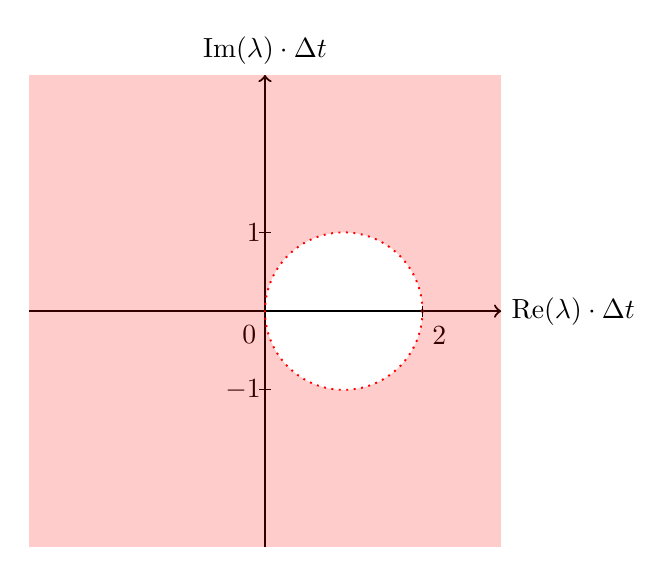
\begin{tikzpicture}
    \draw[thick,->] (-3,0) -- (3,0) node[right] {$\text{Re}(\lambda)\cdot\Delta t$};
    \draw[thick,->] (0,-3) -- (0,3) node[above] {$\text{Im}(\lambda)\cdot\Delta t$};

    \draw[red, dotted, line width=0.7pt] (1,0) circle (1);
    \def\firstcircle{(1,0) circle (1)};
    \draw (2 ,2pt) -- (2,-2pt) node[anchor=north west] {$2$};
    \node at (-0.2,-0.3) {$0$};

    \draw (-2pt ,1) -- (2pt,1) node[left] {$1$};
    \draw (-2pt ,-1) -- (2pt,-1) node[left] {$-1$};
    %\draw[fill=red,red, draw opacity=0.2, fill opacity=0.2] (3,3) rectangle (-3,-3);
    \begin{scope}[even odd rule]% first circle without the second
                \clip \firstcircle (-3,-3) rectangle (3,3);
            \fill[red, fill opacity=0.2] (3,3) rectangle (-3,-3);
    \end{scope}
\end{tikzpicture}

\end{document}
